% !TEX root = ../ts_notes.tex
\documentclass[12pt,fleqn]{article}
\usepackage{../vkCourseML}
\newcounter{chapter}
\hypersetup{unicode=true}
%\usepackage[a4paper]{geometry}
% \usepackage[hyphenbreaks]{breakurl}  % Not needed with pdflatex
\interfootnotelinepenalty=10000
\newcommand{\dx}[1]{\,\mathrm{d}#1} % маленький отступ и прямая d

\begin{document}
\setcounter{figure}{0}
\counterwithin{figure}{chapter}

\section{Deep Learning для временных рядов}

Нейросетевые модели для временных рядов удобно воспринимать как продолжение табличного подхода, но с неявным построением признаков.
Вместо того чтобы вручную задавать лаги, окна, агрегаты и взаимодействия, мы задаём архитектуру, которая может извлекать полезные представления из последовательности.
Цена этой гибкости -- более сложное обучение, больший риск переобучения и более высокие требования к объёму данных.

В прикладном прогнозировании deep learning редко стоит рассматривать как автоматическую замену классических моделей.
Сильные бейзлайны вроде ETS, ARIMA, регрессий на лагах и градиентного бустинга остаются обязательной точкой сравнения, так как модели глубокого обучения не всегда дают сопоставимое качество даже при наличии большого датасета.
Нейросетевой подход обычно имеет смысл, когда рядов много, частота наблюдений высокая или нужно обучить одну глобальную модель на коллекции похожих рядов.

\section{Постановка задачи}

Для последовательных моделей также полезно заранее понимать, какой тип связи между входом и выходом нужен в задаче.
В терминах RNN-архитектур обычно различают несколько схем входов и выходов \cite{arora2024}.
В задачах временных рядов они читаются следующим образом.

\textbf{One-to-many} означает, что из одного фиксированного входа нужно получить целую траекторию.
Например, по одному стартовому значению $y_T$ можно сгенерировать типовую будущую траекторию ряда.
Такая постановка встречается реже, чем обычное прогнозирование по прошлой истории, но полезна для генерации сценариев или типовых профилей.

\textbf{Many-to-one} означает, что всё окно ряда сворачивается в один выход.
Это может быть прогноз на один шаг $\hat{y}_{T+1}$, класс состояния оборудования по последним измерениям или вероятность того, что в ближайшие сутки спрос упадёт ниже порога.
В такой задаче модель должна извлечь из контекста один итоговый признак или одно итоговое число.

\textbf{Many-to-many} с одинаковой длиной входа и выхода означает, что каждому моменту входного окна соответствует свой выход.
Например, можно по ряду измерений датчика получить ряд меток аномалий, восстановить пропущенные значения или построить сглаженную версию сигнала на той же временной сетке.
Это скорее задача разметки, фильтрации или восстановления ряда, чем классический forecast за пределы наблюдаемого окна.

\textbf{Many-to-many} с разной длиной входа и выхода соответствует encoder-decoder или seq2seq-постановке.
В forecasting это самая естественная форма: модель читает прошлое окно длины $k$ и выдаёт будущую траекторию длины $h$, причём $h$ не обязан совпадать с $k$.
Например, по 90 дням продаж можно прогнозировать следующие 14 дней, а по 168 часам нагрузки -- следующие 24 часа.
Дальше в этой главе мы в основном будем относиться именно к этой постановке: по прошлой последовательности строить будущую последовательность другой длины.

Пусть у нас есть временной ряд $(y_t)_{t=1}^{T}$.
Для горизонта $h$ можно рассматривать модель
\begin{equation}
  \hat{y}_{T+1:T+h} = f_\theta(y_{1:T}),
\end{equation}
где $\theta$ обозначает обучаемые параметры нейросети.
В отличие от классических моделей, функция $f_\theta$ обычно не задаётся одной простой формулой.
Она строится как композиция слоёв, нелинейностей и механизмов агрегации информации по времени.

На практике вход почти всегда ограничивают последним окном длины $k$:
\begin{equation}
  \hat{y}_{T+1:T+h} = f_\theta(y_{T-k+1:T}).
\end{equation}
Такое окно называют контекстом.
Слишком короткий контекст может потерять важную сезонность или медленную динамику.
Слишком длинный контекст увеличивает стоимость обучения и может добавить шум.

\section{Глобальные и локальные модели}

Локальная модель обучается отдельно для одного ряда.
Такой подход похож на классические методы и удобен, когда рядов мало или каждый ряд имеет уникальную структуру.
Однако для нейросетей локальное обучение часто оказывается нестабильным, потому что параметров много, а наблюдений в одном ряду может быть недостаточно.

Глобальная модель обучается сразу на множестве рядов.
В этом случае разные ряды дают модели больше примеров, а параметры разделяются между задачами.
Например, одна модель может прогнозировать продажи тысяч товаров, используя только прошлую динамику каждого ряда.
Именно глобальная постановка часто делает deep learning конкурентоспособным в задачах временных рядов.

\section{Основные архитектуры}

\subsection{MLP}

Самый простой переход от табличных моделей к deep learning -- это MLP.
Фактически мы берём уже знакомую табличную задачу с лагами и заменяем модель на полносвязную нейросеть.
Вместо линейной регрессии, случайного леса или бустинга будем оценивать функцию $f_\theta$:
\begin{equation}
  [\hat{y}_{t+h}, \ldots, \hat{y}_{t+1}] = f_\theta(y_t, \ldots, y_{t-k+1}), \quad t \in \overline{k, T-h}.
\end{equation}

Постановка остаётся ровно такой же, как в MIMO-стратегии.
Мы подаём на вход окно прошлых значений и сразу получаем вектор прогнозов на весь горизонт.

\begin{figure}[!h]
  \centering
  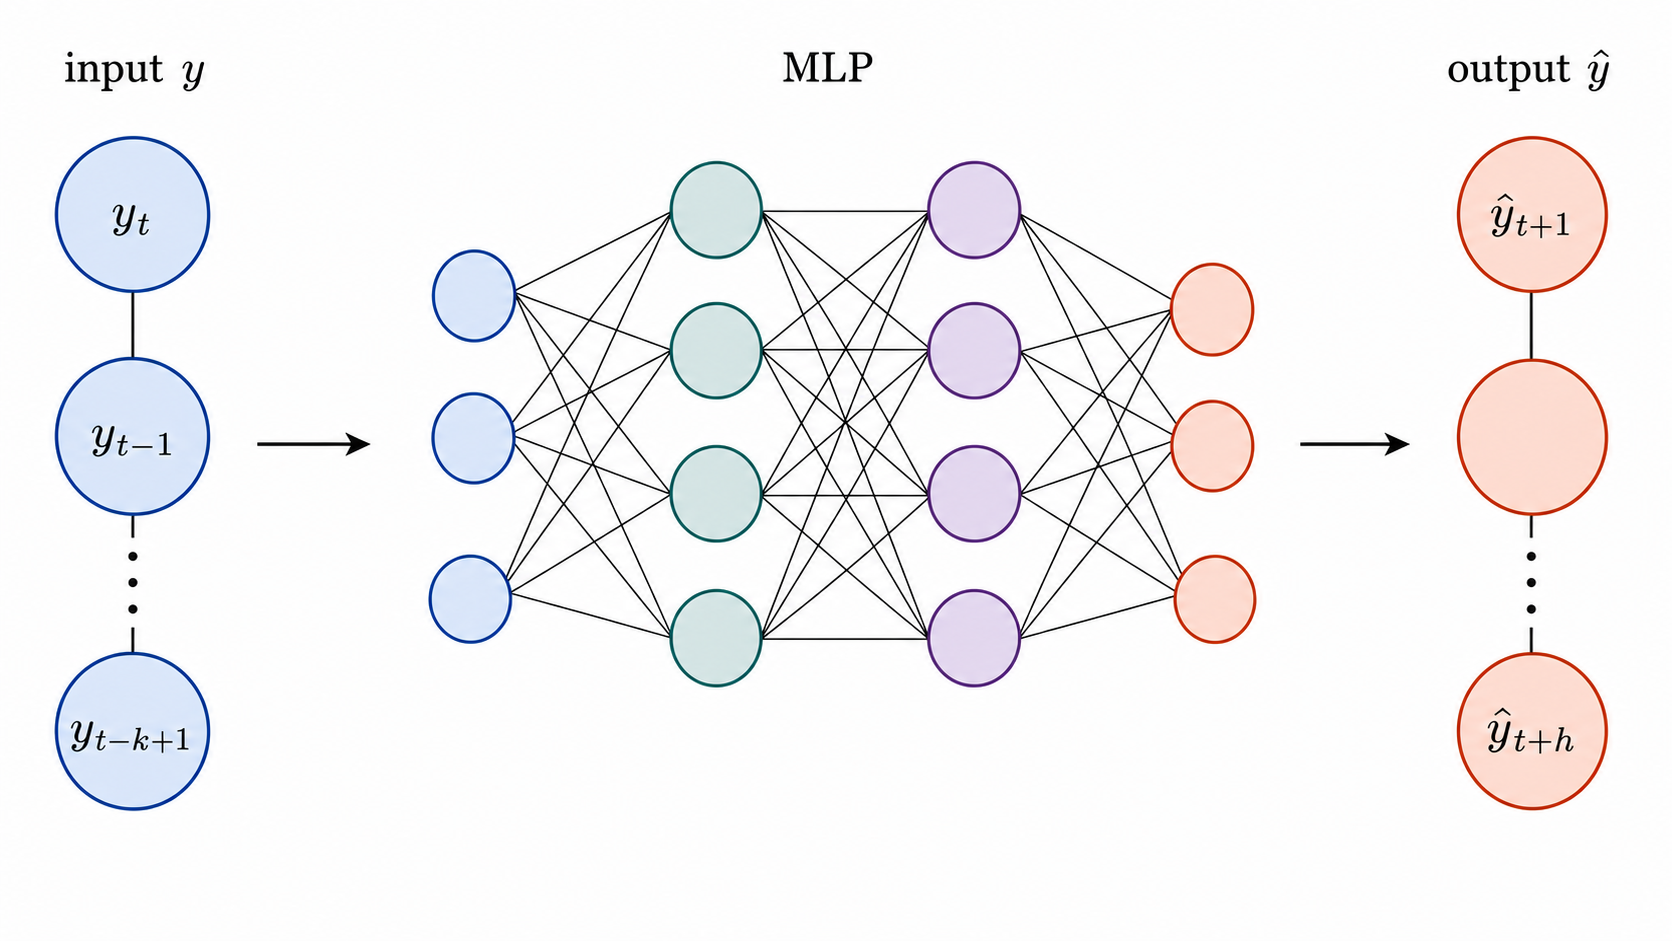
\includegraphics[width=0.95\linewidth]{images/04_deep_learning_mlp.png}
  \caption{MLP как прямой нейросетевой аналог MIMO-стратегии.}
\end{figure}

Такой подход удобен как простой нейросетевой бейзлайн.

\subsection{RNN}

Рекуррентные нейросети возникли как попытка перенести идею нейросетевого моделирования с фиксированных векторов на последовательности.
Обычная MLP видит только заранее заданное окно лагов и не имеет собственного состояния.
RNN, наоборот, обрабатывает ряд по шагам и на каждом шаге переносит вперёд скрытое состояние.
В этом смысле скрытое состояние можно понимать как сжатую память о прошлом ряда.

\begin{figure}[!h]
  \centering
  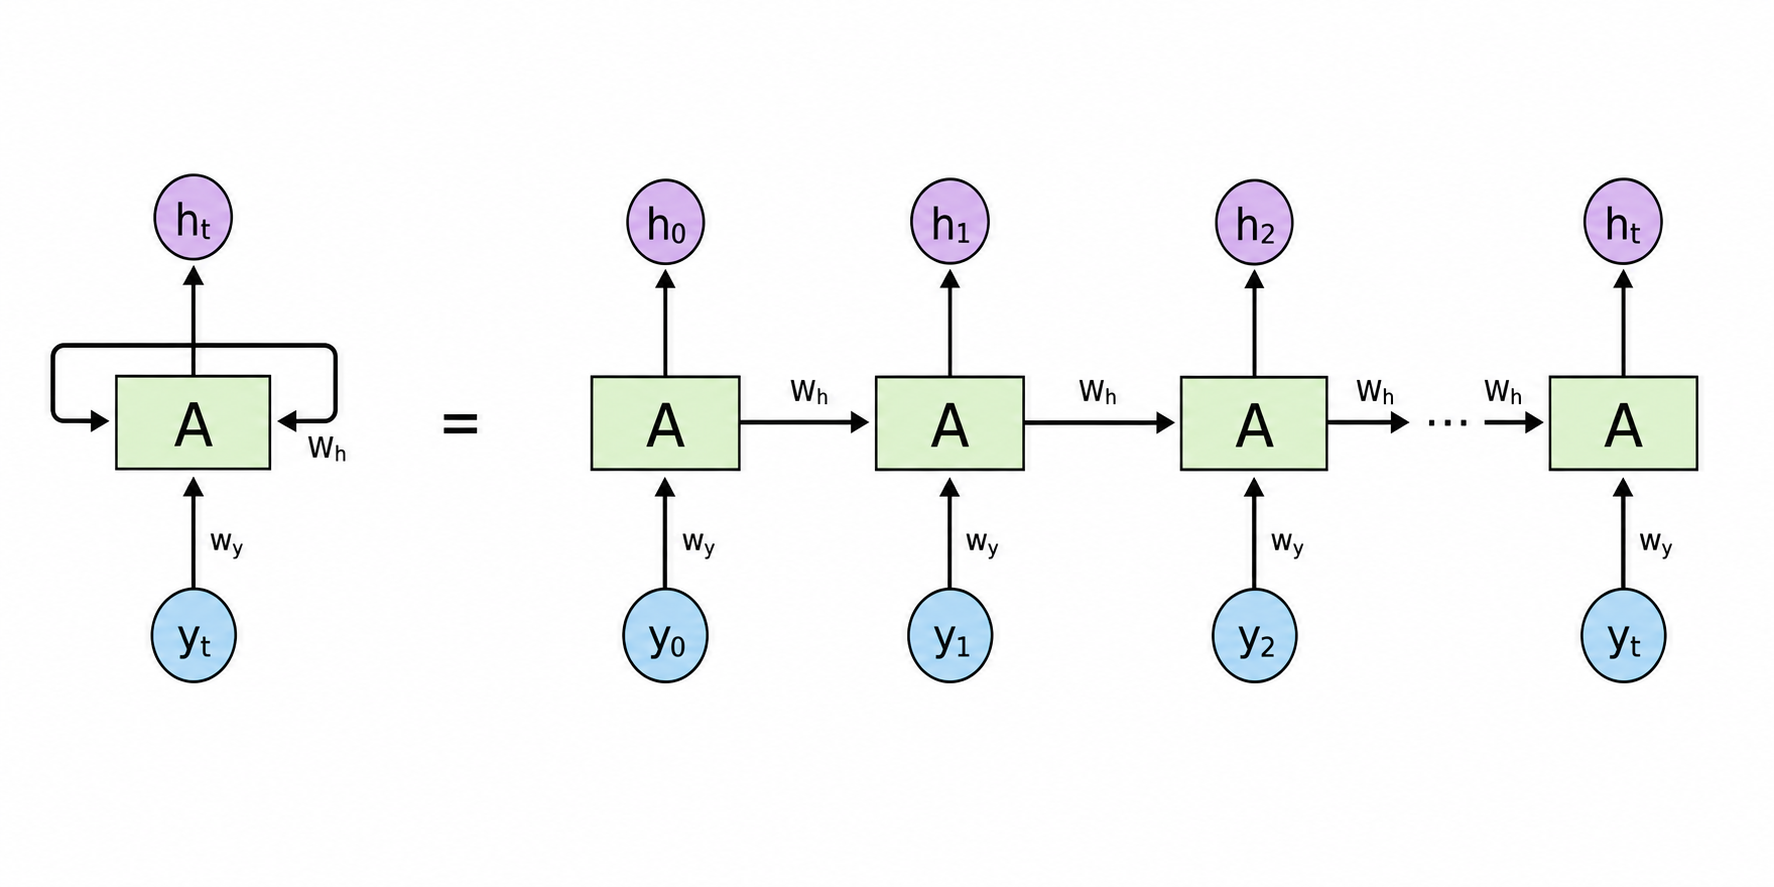
\includegraphics[width=0.95\linewidth]{images/04_deep_learning_rnn_unrolled.png}
  \caption{Развёртка одной и той же рекуррентной ячейки по времени.}
\end{figure}

На схеме каждая зелёная ячейка обозначена одной буквой $A$, потому что это не разные слои со своими параметрами, а одна и та же функция обновления состояния.
В развёртке на каждом шаге повторно используются одни и те же веса входа $w_y$, рекуррентная матрица $W_h$ и смещение $b_h$.
Меняются только текущее значение ряда $y_t$ и скрытое состояние $h_t$.

Исторически важной простой формой такой модели стала simple recurrent network Элмана.
В ней предыдущее скрытое состояние копируется в следующий момент времени и вместе с текущим входом участвует в вычислении нового состояния.
Для временных рядов это естественная идея: прогноз зависит не только от текущего значения $y_t$, но и от внутреннего состояния, накопленного при просмотре предыдущих наблюдений.

Формально пусть на шаге $t$ модель получает значение ряда $y_t$ и хранит скрытое состояние $h_t \in \mathbb{R}^{m}$.
Простейшую RNN можно записать как
\begin{equation}
  h_t = \phi(w_y y_t + W_h h_{t-1} + b_h),
\end{equation}
где $w_y$ отвечает за вход ряда, $W_h$ отвечает за перенос прошлого состояния, а $\phi$ является нелинейной функцией активации.
Прогноз на один шаг можно получить из скрытого состояния:
\begin{equation}
  \hat{y}_{t+1} = g_\theta(h_t).
\end{equation}
На этом уровне RNN задаёт только способ обновления скрытого состояния.
Стратегия получения нескольких будущих значений выбирается отдельно и обсуждается в следующем подразделе.

Главная слабая сторона такой модели состоит в том, что вся история ряда должна быть сжата в один вектор $h_t$ фиксированной размерности.
Если зависимость короткая, этого может быть достаточно.
Если важный сигнал находится далеко в прошлом, простая RNN часто не умеет устойчиво сохранить его до момента прогноза.
На длинных последовательностях это приводит к слабой работе с долгосрочными зависимостями и делает модель чувствительной к выбору длины контекста.
В работе Lai et al. по forecasting для Solar Energy, Traffic и Electricity простой рекуррентный бейзлайн работал заметно хуже модели, где периодические связи в рядах учитывались явно \cite{lai2018}.
Это хороший эмпирический пример того, что одной внутренней памяти часто недостаточно, если в ряду есть суточные, недельные или другие длинные повторяющиеся паттерны.
Увеличение размерности $h_t$ повышает ёмкость модели, но само по себе не убирает фиксированное узкое место.

На практике это означает, что vanilla RNN редко является сильной финальной моделью для сложного прогнозирования.
Её удобно использовать как учебную архитектуру и как первый шаг к gated-моделям.
Именно ограничения простой RNN мотивируют переход к LSTM и GRU, где памятью управляют специальные механизмы.

\subsection{Backpropagation through time}
\label{sec:bptt}

Обучение RNN сложнее, чем обучение обычной MLP, потому что одни и те же параметры используются на каждом временном шаге.
Чтобы посчитать градиенты, модель разворачивают по времени и применяют backpropagation through time.
После такого разворачивания одна рекуррентная ячейка превращается в глубокую сеть, где каждый слой соответствует своему моменту времени.


Рассмотрим vanilla RNN на одном обучающем окне.
Для простоты будем считать, что ряд одномерный, а модель на каждом шаге строит прогноз следующего значения:
\begin{align}
  a_t &= w_y y_t + W_h h_{t-1} + b_h,
  &
  h_t &= \phi(a_t),
  \\
  \hat{y}_{t+1} &= v^\top h_t + b_o,
  &
  t &\in \overline{1, T-1}.
\end{align}
Здесь $a_t$ -- предактивация, $h_t$ -- скрытое состояние, $w_y$ -- вектор весов для входа ряда, $W_h$ -- матрица рекуррентного перехода, а $v$ и $b_o$ задают выходной слой.
Возьмём квадратичную функцию потерь по всему окну:
\begin{equation}
  L
  =
  \frac{1}{2}
  \sum_{t=1}^{T-1}
  (\hat{y}_{t+1} - y_{t+1})^2.
\end{equation}
Обозначим ошибку прогноза на шаге $t$ через
\begin{equation}
  \varepsilon_t
  =
  \frac{\partial L}{\partial \hat{y}_{t+1}}
  =
  \hat{y}_{t+1} - y_{t+1}.
\end{equation}
Тогда градиенты выходного слоя считаются так же, как в обычной нейросети:
\begin{align}
  \frac{\partial L}{\partial v}
  &=
  \sum_{t=1}^{T-1}
  \varepsilon_t h_t,
  &
  \frac{\partial L}{\partial b_o}
  &=
  \sum_{t=1}^{T-1}
  \varepsilon_t.
\end{align}

Главная особенность BPTT появляется при вычислении градиентов по рекуррентной части.
Состояние $h_t$ влияет на loss двумя путями.
Первый путь прямой: через прогноз $\hat{y}_{t+1}$ на текущем шаге.
Второй путь рекуррентный: через следующее состояние $h_{t+1}$, затем через $h_{t+2}$ и так далее.
Поэтому ошибку нужно переносить назад по времени.

Введём величину
\begin{equation}
  \delta_t
  =
  \frac{\partial L}{\partial a_t}.
\end{equation}
Она показывает, какой градиент пришёл в предактивацию рекуррентной ячейки на шаге $t$.
Обратный проход начинается с конца окна.
Если после шага $T-1$ состояния уже не участвуют в loss, удобно положить $\delta_T = 0$.
Для $t = T-1, T-2, \ldots, 1$ получаем рекурсию
\begin{align}
  \frac{\partial L}{\partial h_t}
  &=
  \varepsilon_t v + W_h^\top \delta_{t+1},
  \\
  \delta_t
  &=
  \left(
    \varepsilon_t v + W_h^\top \delta_{t+1}
  \right)
  \odot
  \phi^\prime(a_t).
\end{align}
Первое слагаемое $\varepsilon_t v$ приходит от текущего прогноза.
Второе слагаемое $W_h^\top \delta_{t+1}$ приходит из будущего состояния.
Именно эта рекурсия делает backpropagation «through time»: градиент от будущих ошибок проходит назад через одну и ту же матрицу $W_h$.

После того как все $\delta_t$ найдены, градиенты параметров рекуррентной ячейки получаются суммированием вкладов всех временных шагов:
\begin{align}
  \frac{\partial L}{\partial W_h}
  &=
  \sum_{t=1}^{T-1}
  \delta_t h_{t-1}^\top,
  \\
  \frac{\partial L}{\partial w_y}
  &=
  \sum_{t=1}^{T-1}
  \delta_t y_t,
  \\
  \frac{\partial L}{\partial b_h}
  &=
  \sum_{t=1}^{T-1}
  \delta_t.
\end{align}
Сумма появляется потому, что одни и те же $W_h$, $w_y$ и $b_h$ используются на каждом шаге развёртки.
То есть BPTT -- это обычное дифференцирование вычислительного графа, но с обязательным учётом совместного использования параметров во времени.

Теперь видно, откуда берутся vanishing и exploding gradients.
Если посмотреть на влияние состояния $h_s$ на более позднее состояние $h_t$, то по правилу цепочки
\begin{equation}
  \frac{\partial h_t}{\partial h_s}
  =
  \prod_{i=s+1}^{t}
  D_i W_h,
  \quad
  D_i = \mathrm{diag}\!\left(\phi^\prime(a_i)\right).
\end{equation}
Градиент многократно проходит через матрицу перехода $W_h$ и производные активаций.
Поэтому его норма ведёт себя как произведение многих матриц.
Если типичный множитель меньше единицы, вклад далёкого прошлого убывает почти экспоненциально.
Если типичный множитель больше единицы, градиент может резко вырасти.
На временных рядах этот эффект проявляется особенно заметно, когда важный лаг равен суткам, неделе или другому длинному периоду.
Lai et al. прямо связывают трудность off-the-shelf GRU и LSTM с затуханием градиента и добавляют skip-связь $h_{t-p} \to h_t$, где для часовых Traffic и Electricity берут $p=24$ \cite{lai2018}.
Именно эту общую механику Pascanu, Mikolov и Bengio используют для объяснения vanishing и exploding gradients и показывают, почему простое gradient clipping является практичным способом бороться со взрывом градиента \cite{pascanu2013}.

На практике BPTT часто ограничивают последними $k$ шагами.
Такой вариант называют truncated BPTT.
Он снижает стоимость обучения и уменьшает длину произведения матриц, но одновременно ограничивает то, как далеко назад во времени loss может напрямую передать градиент.

\subsection{Варианты декодинга для multi-step forecasting}
\label{sec:rnn-decoding}

Рекуррентная ячейка и стратегия прогноза на несколько шагов -- это разные решения.
RNN, LSTM или GRU определяют, как обновляется скрытое состояние, но не навязывают один обязательный способ получить $\hat{y}_{t+1:t+h}$.
На практике для временных рядов чаще всего встречаются три сценария.

\textbf{Direct multi-horizon} или MIMO-стратегия сразу возвращает весь вектор будущих значений:
\begin{equation}
  [\hat{y}_{t+1}, \ldots, \hat{y}_{t+h}] = g_\theta(h_t).
\end{equation}
Такую постановку удобно использовать, когда горизонт $h$ фиксирован заранее.
Loss считается по всему горизонту, поэтому модель учится прогнозировать не только ближайший шаг, но и дальние точки траектории.
В классической литературе по multi-step forecasting MIMO-стратегия важна потому, что сохраняет зависимость между будущими значениями и не требует рекурсивно подставлять собственные ошибки обратно во вход \cite{bentaieb2012}.
В нейросетевых моделях близкую идею использует MQ-RNN: авторы прямо мотивируют direct multi-horizon forecast тем, что рекурсивный подход может накапливать ошибки на длинном горизонте \cite{wen2017}.

\begin{figure}[htbp]
  \centering
  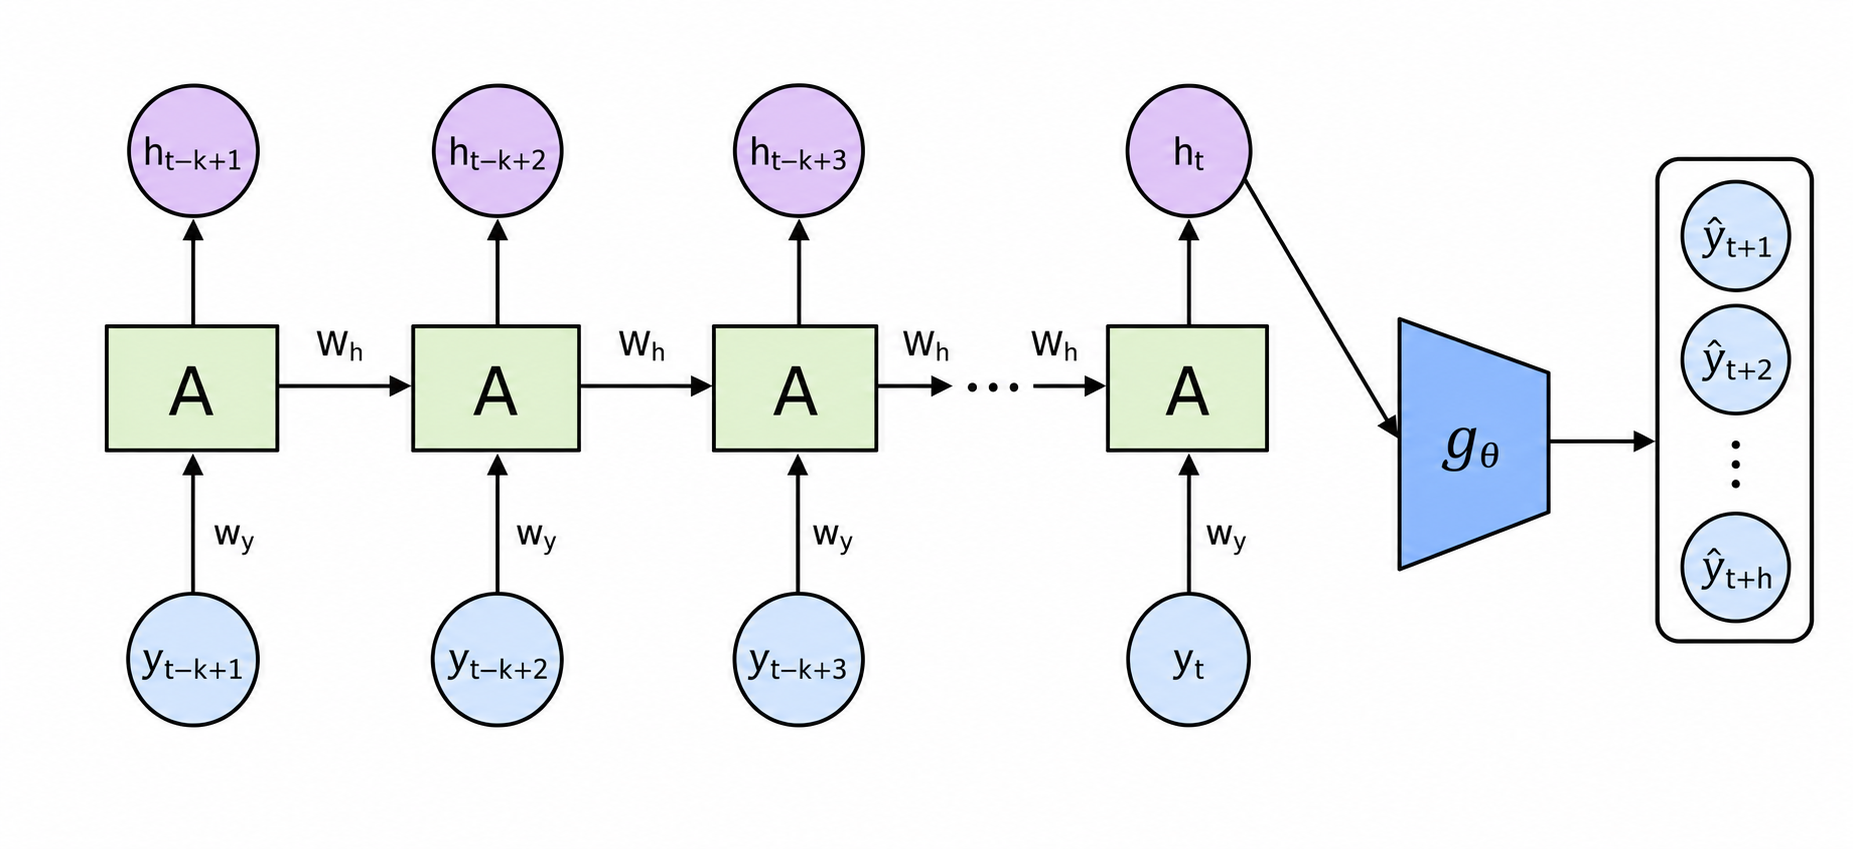
\includegraphics[width=0.95\linewidth]{images/04_deep_learning_direct_multi_horizon.png}
  \caption{Direct multi-horizon подход: последняя скрытая переменная $h_t$ передаётся в голову $g_\theta$, которая сразу возвращает вектор прогнозов $\hat{y}_{t+1:t+h}$.}
  \label{fig:deep_learning_direct_multi_horizon}
\end{figure}

\textbf{Рекурсивная} или autoregressive-стратегия сначала строит прогноз на один шаг, а затем использует этот прогноз как вход для следующего искусственного шага развёртки:
\begin{align}
  \hat{h}_{t+1} &= \phi(w_y \hat{y}_{t+1} + W_h h_t + b_h),
  &
  \hat{y}_{t+2} &= g_\theta(\hat{h}_{t+1}),
  \\
  \hat{h}_{t+2} &= \phi(w_y \hat{y}_{t+2} + W_h \hat{h}_{t+1} + b_h),
  &
  \hat{y}_{t+3} &= g_\theta(\hat{h}_{t+2}).
\end{align}
Дальше те же преобразования повторяются до горизонта $h$.
Важно, что здесь нет отдельного decoder-модуля.
Мы берём уже обученную рекуррентную ячейку и выходной слой для one-step forecasting, а затем рекурсивно применяем их к собственным прогнозам.
Поэтому такая стратегия проста и экономна по параметрам, но ошибки прогноза могут накапливаться вдоль горизонта.
Зато autoregressive-декодинг естественен для вероятностного forecasting, где нужно генерировать согласованные sample paths.
Например, DeepAR обучает авторегрессионную RNN на множестве связанных рядов, а в prediction range подаёт сэмплированное будущее значение обратно в модель для следующего шага \cite{salinas2017}.

\begin{figure}[htbp]
  \centering
  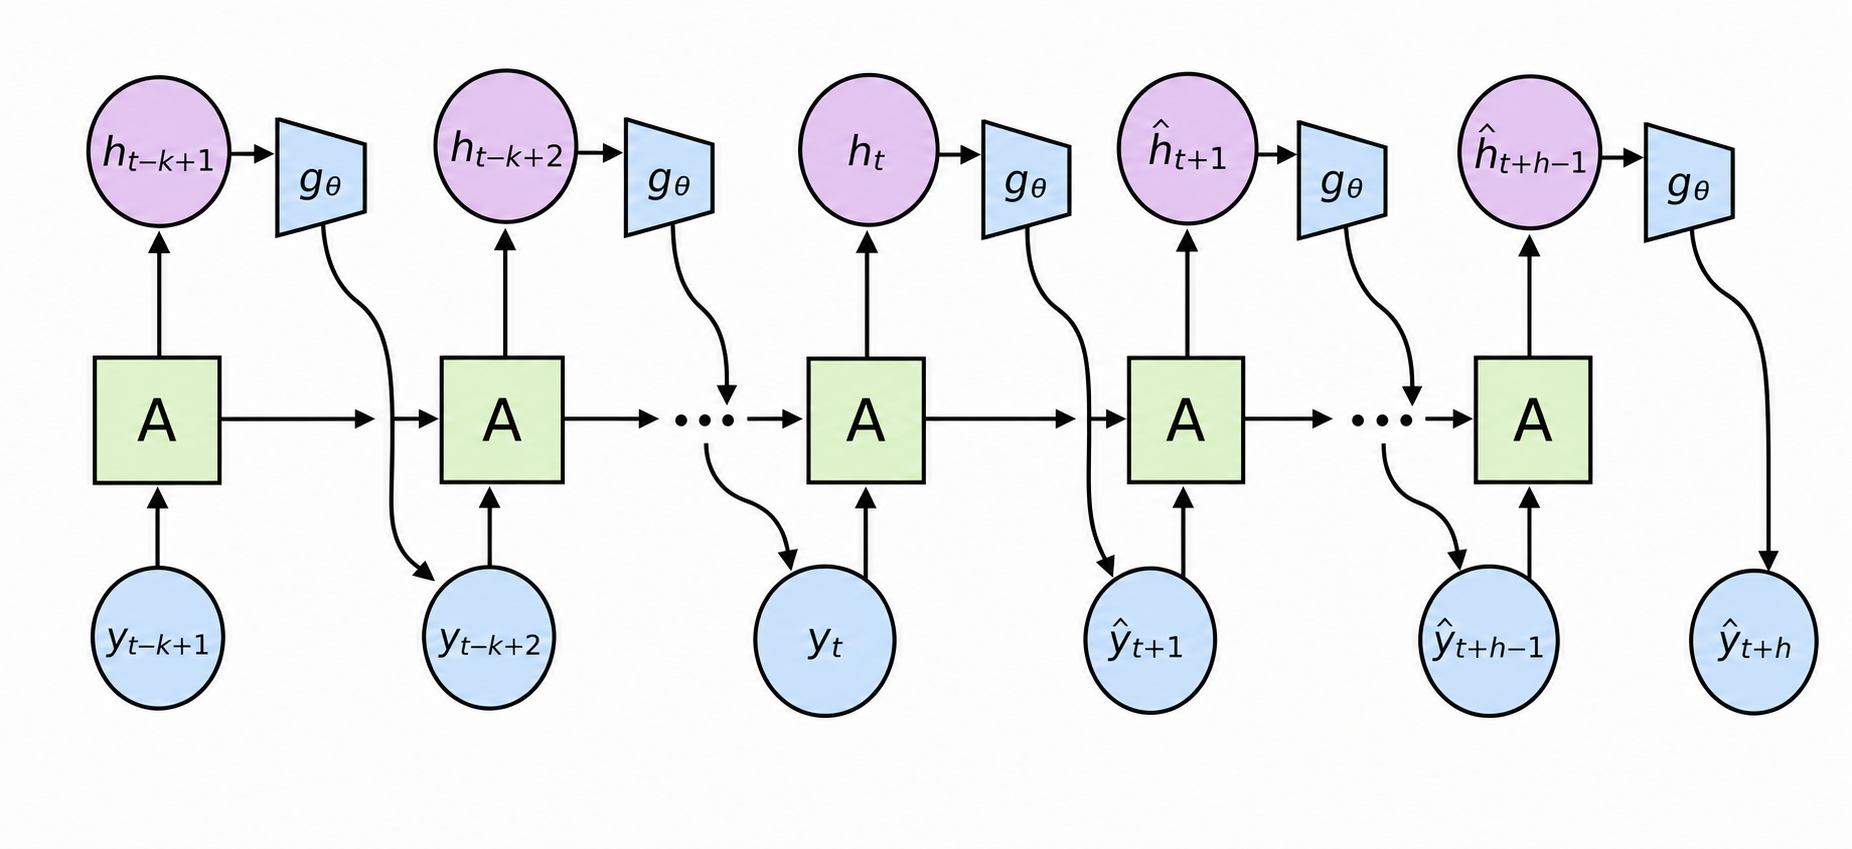
\includegraphics[width=0.95\linewidth]{images/04_deep_learning_recursive_strategy.png}
  \caption{Рекурсивная стратегия: голова $g_\theta$ на каждом шаге выдаёт один прогноз $\hat{y}$, который затем используется как вход следующей искусственной ячейки.}
  \label{fig:deep_learning_recursive_strategy}
\end{figure}

\textbf{Seq2Seq encoder-decoder} разделяет модель на encoder и decoder.
Encoder читает прошлое окно и сжимает его в скрытое состояние, а decoder порождает будущую последовательность.
Обычно это две разные рекуррентные ячейки со своими параметрами: одна ячейка отвечает за кодирование прошлой последовательности, другая -- за генерацию будущей.
Начальное состояние decoder получают из последнего состояния encoder, но дальше decoder разворачивается уже как отдельная рекуррентная сеть.
Схематично это можно записать как
\begin{align}
  h_t^{\mathrm{enc}} &= \mathrm{RNN}_{\mathrm{enc}}(y_t, h_{t-1}^{\mathrm{enc}}),
  &
  s_0 &= h_T^{\mathrm{enc}},
  \\
  s_1 &= \mathrm{RNN}_{\mathrm{dec}}(y_T, s_0),
  &
  \hat{y}_{T+1} &= g_\theta(s_1),
  \\
  s_j &= \mathrm{RNN}_{\mathrm{dec}}(\hat{y}_{T+j-1}, s_{j-1}),
  &
  \hat{y}_{T+j} &= g_\theta(s_j),
  \quad j \in \overline{2, h}.
\end{align}
Во время обучения decoder часто получает предыдущее истинное значение ряда, а во время прогноза -- предыдущее предсказанное значение.
Decoder может идти шаг за шагом, но функция потерь обычно считается по всему будущему горизонту.
Поэтому seq2seq находится между чисто рекурсивным и чисто direct-подходом: он порождает траекторию последовательно, но обучается как задача прогноза всей будущей последовательности.

\subsection{LSTM}

LSTM можно понимать как ответ на главный недостаток простой RNN: ей трудно долго и устойчиво хранить информацию в одном скрытом состоянии.
Если у vanilla RNN память обновляется одним преобразованием $h_t = \phi(w_y y_t + W_h h_{t-1} + b_h)$, то LSTM разделяет память на два потока.
Первый поток -- это скрытое состояние $h_t$, которое отдаётся наружу и используется для прогноза.
Второй поток -- это состояние ячейки $c_t$, которое специально устроено так, чтобы информация могла проходить через много шагов с меньшими потерями.

Идея LSTM была предложена Hochreiter и Schmidhuber как способ поддерживать почти постоянный поток ошибки внутри специальных ячеек памяти \cite{hochreiter1997}.
В современной записи обычно используют три управляющих фильтра: фильтр забывания, входной фильтр и выходной фильтр.
Forget gate появился позже: Gers, Schmidhuber и Cummins добавили его, чтобы ячейка могла сама сбрасывать устаревшую память в непрерывных потоках данных \cite{gers2000}.
Именно эта версия стала стандартной.
Хорошее визуальное объяснение такой ячейки есть в статье Christopher Olah, перевод которой опубликован на Хабре \cite{olah2017habr}.


Пусть на шаге $t$ модель получает значение ряда $y_t$.
Тогда типичная LSTM-ячейка задаётся уравнениями
\begin{align}
  f_t &= \sigma(W_f [h_{t-1}, y_t] + b_f),
  &
  i_t &= \sigma(W_i [h_{t-1}, y_t] + b_i),
  \\
  \widetilde{c}_t &= \tanh(W_c [h_{t-1}, y_t] + b_c),
  &
  c_t &= f_t \odot c_{t-1} + i_t \odot \widetilde{c}_t,
  \\
  o_t &= \sigma(W_o [h_{t-1}, y_t] + b_o),
  &
  h_t &= o_t \odot \tanh(c_t).
\end{align}
Здесь $\sigma$ возвращает значения от нуля до единицы, а $\odot$ означает покомпонентное умножение.
Фильтр забывания $f_t$ решает, какую часть старой памяти $c_{t-1}$ оставить.
Входной фильтр $i_t$ решает, какую часть нового кандидата $\widetilde{c}_t$ записать в память.
Выходной фильтр $o_t$ решает, какую часть памяти показать наружу через скрытое состояние $h_t$.


Такое устройство решает сразу несколько проблем простой RNN.
Во-первых, градиенту больше не обязательно каждый раз проходить через одну и ту же нелинейность скрытого состояния.
Вдоль состояния ячейки есть аддитивная связь $c_t = f_t \odot c_{t-1} + \ldots$, поэтому модель может научиться держать $f_t$ близким к единице и сохранять важную информацию много шагов подряд.
Во-вторых, модель получает явный механизм перезаписи памяти.
Для временных рядов это важно, когда старый режим больше не актуален: например, после смены уровня спроса, изменения тарифа, релиза продукта или календарного события.
В-третьих, LSTM разделяет вопрос «что хранить?» и вопрос «что отдавать в прогноз?».
Это полезно, если память о далёком событии нужна позже, но не должна искажать каждый промежуточный прогноз.

\subsubsection{Constant Error Carousel}

Ключевая идея LSTM в том, что у модели есть отдельная дорога для памяти -- состояние ячейки $c_t$.
В оригинальной статье эту дорогу называли constant error carousel, или CEC \cite{hochreiter1997}.
В той версии ячейка имела линейную recurrent-связь с самой собой с весом $1$.
Поэтому, если входной и выходной gates не мешали, ошибка при обратном проходе могла циркулировать внутри ячейки почти без изменения масштаба.
Смысл названия простой: если информация уже записана в память, ошибка не обязана каждый раз проходить через обычную нелинейность скрытого состояния.
Именно это помогает LSTM хранить долгосрочные зависимости лучше, чем vanilla RNN.

В vanilla RNN память обновляется как
\begin{equation}
  h_t = \phi(w_y y_t + W_h h_{t-1} + b_h).
\end{equation}
Чтобы градиент от $h_t$ дошёл до $h_{t-1}$, он проходит через производную $\phi^\prime$ и матрицу $W_h$.
На длинной последовательности такие множители повторяются много раз, поэтому градиент легко затухает или взрывается.

В LSTM состояние ячейки обновляется иначе:
\begin{equation}
  c_t = f_t \odot c_{t-1} + i_t \odot \widetilde{c}_t.
\end{equation}
В современной LSTM старое состояние $c_{t-1}$ входит в новое состояние $c_t$ почти напрямую, но уже через покомпонентное умножение на forget gate $f_t$.
То есть постоянный коэффициент self-связи из исходного CEC заменён адаптивным коэффициентом $f_t$.
Если $f_t$ близок к единице, то модель почти копирует старую память:
\begin{equation}
  c_t \approx c_{t-1} + i_t \odot \widetilde{c}_t.
\end{equation}
Это означает, что важная информация может идти по времени как по почти прямому каналу.
Модель не обязана заново пересчитывать всю память из $h_{t-1}$ и $y_t$ на каждом шаге.

То же самое видно в градиентах.
Если временно считать фильтры фиксированными, то
\begin{equation}
  \frac{\partial c_t}{\partial c_{t-1}}
  \approx
  \mathrm{diag}(f_t).
\end{equation}
Для нескольких шагов назад получаем
\begin{equation}
  \frac{\partial c_t}{\partial c_s}
  \approx
  \prod_{i=s+1}^{t}
  \mathrm{diag}(f_i).
\end{equation}
Если компоненты $f_i$ близки к единице, это произведение не исчезает быстро.
Поэтому градиент может дойти от далёкого будущего loss к далёкому прошлому состоянию ячейки.
В этом и состоит практический смысл constant error carousel: LSTM может научиться держать «дверь памяти» открытой столько шагов, сколько нужно.
Но после добавления forget gate эта дверь больше не открыта автоматически: её начальное положение задаётся bias и затем меняется обучением.

Поэтому этот механизм сильно зависит от того, с каких значений стартуют gates.
Если forget gate в начале обучения часто выдаёт значения около нуля, то состояние ячейки будет стираться почти сразу:
\begin{equation}
  f_t \approx 0
  \quad \Rightarrow \quad
  c_t \approx i_t \odot \widetilde{c}_t.
\end{equation}
Тогда CEC практически не работает: градиент по $c_t$ не может долго идти назад по времени, потому что путь через $c_{t-1}$ закрыт.
Поэтому на практике bias forget gate часто инициализируют положительным числом.
Эмпирическое исследование Jozefowicz, Zaremba и Sutskever показывает, что добавление bias $1$ к forget gate заметно улучшает обычную LSTM и сокращает разрыв с GRU \cite{jozefowicz2015}.
Например, если в начале обучения входы в сигмоиду малы, то
\begin{equation}
  f_t
  =
  \sigma(W_f [h_{t-1}, y_t] + b_f)
  \approx
  \sigma(b_f).
\end{equation}
При $b_f = 0$ получаем $\sigma(b_f) = 0.5$, и память на каждом шаге уже наполовину затухает.
При $b_f = 1$ получаем $\sigma(b_f) \approx 0.73$, поэтому начальное затухание становится медленнее.
Это не гарантирует долгую память само по себе, но даёт модели более благоприятную стартовую точку: сначала она склонна сохранять память, а затем во время обучения может научиться забывать там, где это полезно.

Более точная идея той же природы называется chrono initialization \cite{tallec2018}.
Она связывает bias gates с ожидаемой длиной зависимостей в данных.
Если hidden size равен $n$, то chrono initialization сэмплирует отдельный начальный масштаб для каждой координаты состояния:
\begin{equation}
  r_j \sim U(1, T_{\max} - 1),
  \qquad
  b_{f,j} = \log r_j,
  \qquad
  b_{i,j} = -b_{f,j},
  \qquad
  j = 1,\ldots,n.
\end{equation}
Иными словами, $b_f$ и $b_i$ -- это bias-векторы, а не один общий скаляр на весь gate.
Одна координата ячейки может стартовать с короткой памятью, другая -- с более длинной.
Это важно, потому что chrono initialization задаёт набор начальных временных масштабов, а не один общий масштаб для всей LSTM.
Она не сэмплирует элементы матриц $W_f$, $W_i$ или recurrent-весов; речь идёт именно о компонентах bias-векторов gates.
Тогда в начале обучения
\begin{equation}
  f_{t,j} \approx \sigma(b_{f,j}) = \frac{r_j}{1 + r_j}.
\end{equation}
Большие значения $r_j$ дают $f_{t,j}$ ближе к единице и более медленное забывание.
Отрицательный bias входного gate $b_i$ одновременно уменьшает раннюю запись новой информации, чтобы новая память не перезаписывала старую слишком агрессивно.
Иначе говоря, CEC -- это не только архитектурная идея, но и практическая договорённость об инициализации: в начале обучения дверь памяти лучше слегка приоткрыть и настроить её под ожидаемый масштаб ряда.

Важно, что LSTM не отменяет проблему затухания градиентов полностью.
Если forget gate долго держится около нуля, старая информация всё равно стирается.
Но теперь это не только побочный эффект матричных произведений, а управляемое решение модели.
Она может забыть старый режим ряда, когда он больше не нужен, или сохранить долгую сезонную информацию, если она полезна для прогноза.

Для прогноза на несколько шагов LSTM используют те же сценарии декодинга, что и для обычной RNN.
Можно сразу вернуть весь горизонт, строить прогноз autoregressive или использовать encoder-decoder схему.
Эти варианты описаны отдельно в подразделе \ref{sec:rnn-decoding}.

Сильная сторона LSTM на временных рядах -- способность обучаться на коллекции похожих рядов и переносить статистическую силу между ними.
Это полезно, когда есть много коротких, но родственных рядов: продажи товаров, нагрузки узлов сети, транзакции клиентов, датчики одного типа.
Например, в M4 Competition победила гибридная модель ES-RNN, где экспоненциальное сглаживание отвечало за уровень и сезонность отдельных рядов, а LSTM использовалась для нелинейной динамики и cross-learning \cite{smyl2020}.
Такой пример хорошо показывает типичную роль LSTM: не чистая замена ETS или ARIMA, а компонент гибридной forecasting-системы.

При этом LSTM не является универсальным решением для forecasting.
Она остаётся рекуррентной моделью, поэтому обучение и inference идут последовательно по времени и хуже параллелятся, чем MLP, CNN/TCN или Transformer-подходы.
Кроме того, LSTM требует аккуратного масштабирования, выбора длины контекста, регуляризации, early stopping и проверки против простых бейзлайнов.
Если данных мало, ряд один, а динамика хорошо описывается уровнем, трендом и сезонностью, ETS, ARIMA или регрессия на лагах могут быть стабильнее и понятнее.
В обзоре Hewamalage, Bergmeir и Bandara подчёркивается, что RNN-модели стали конкурентоспособны в forecasting, но всё ещё уступают классическим методам по автоматичности, робастности и простоте применения для неспециалистов \cite{hewamalage2021}.

Наконец, gated-память не гарантирует, что модель сама найдёт длинную календарную периодичность.
Если важный лаг равен 24, 168 или 365 шагам, на практике часто помогают удаление сезонности, skip-связи или гибрид с авторегрессионным компонентом.
В работе Lai et al. обычные GRU/LSTM были слабыми бейзлайнами, а улучшение давали свёрточная часть, recurrent-skip механизм и авторегрессионная компонента \cite{lai2018}.
Поэтому LSTM особенно уместна как глобальная модель для многих связанных рядов или как часть гибридной системы, а в маленьких задачах с простой сезонностью часто оказывается избыточной.

\subsection{GRU}

GRU, или gated recurrent unit, была предложена Cho et al. как более компактная gated-ячейка для encoder-decoder RNN \cite{cho2014}.
Как и LSTM, она решает проблему простой RNN: модели нужен управляемый способ решать, какую информацию сохранить, какую обновить и когда старое состояние можно почти не трогать.
Но GRU делает это без отдельного состояния ячейки $c_t$.
Вся память хранится в одном скрытом состоянии $h_t$.

В типичной записи GRU использует два gates:
\begin{align}
  z_t &= \sigma(W_z [h_{t-1}, y_t] + b_z),
  &
  r_t &= \sigma(W_r [h_{t-1}, y_t] + b_r),
  \\
  \widetilde{h}_t &= \tanh(W_h [r_t \odot h_{t-1}, y_t] + b_h),
  &
  h_t &= z_t \odot h_{t-1} + (1 - z_t) \odot \widetilde{h}_t.
\end{align}
Здесь $z_t$ -- update gate.
В выбранной записи он задаёт, какую долю старого состояния $h_{t-1}$ оставить в новом состоянии.
Если $z_t$ близок к единице, GRU почти копирует старую память.
Если $z_t$ близок к нулю, модель сильнее переписывает состояние кандидатом $\widetilde{h}_t$.
Reset gate $r_t$ управляет тем, сколько прошлого состояния попадёт в кандидата.
Если $r_t$ мал, кандидат строится почти без опоры на старое $h_{t-1}$, что удобно при смене режима ряда.


Главное отличие от LSTM в том, что GRU объединяет несколько решений в более короткую схему.
У LSTM есть отдельная память $c_t$, hidden state $h_t$, forget gate, input gate и output gate.
У GRU нет отдельного $c_t$ и нет output gate: состояние, которое хранится, сразу является состоянием, которое отдаётся дальше.
Из-за этого GRU обычно имеет меньше параметров, быстрее обучается и может быть устойчивее на небольших данных.
Эмпирическая работа Chung et al. показывает, что GRU и LSTM заметно сильнее простой tanh-RNN на задачах sequence modeling, а различие между GRU и LSTM зависит от данных и настройки модели \cite{chung2014}.

Интуиция для временных рядов такая же, как у LSTM, но чуть проще.
Update gate помогает удерживать уровень, фазу сезонности или медленную динамику, не пересчитывая всё скрытое состояние на каждом шаге.
Reset gate помогает быстрее забывать старую историю, когда ряд переходит в новый режим.
Поэтому GRU удобно пробовать там, где хочется получить gated-память дешевле, чем в LSTM.

Слабые стороны тоже похожи на LSTM.
GRU остаётся рекуррентной моделью, поэтому хуже параллелится по времени, чем CNN/TCN или Transformer-подходы.
Кроме того, из-за отсутствия отдельного состояния ячейки и output gate у неё меньше способов разделить «что хранить?» и «что показывать наружу?».
Если задача требует очень долгой памяти или аккуратного отделения внутреннего состояния от прогноза, LSTM может оказаться выразительнее.
Если же данных мало или сезонность простая, GRU, как и LSTM, может проиграть более простым бейзлайнам по стабильности и интерпретируемости.

Для multi-step forecasting GRU не задаёт отдельную стратегию декодинга.
Как и LSTM, она может использовать direct/MIMO, autoregressive или encoder-decoder сценарий из подраздела \ref{sec:rnn-decoding}.

\subsection{Эмбеддинги временных рядов}

В NLP embedding обычно начинается с дискретного токена: слово или subword превращается в индекс, а индекс -- в вектор из обучаемой таблицы.
Для временного ряда такой естественной таблицы нет.
Значения $y_t$ непрерывные, масштаб зависит от ряда, а смысл наблюдения часто определяется не только самим числом, но и его соседями, позицией в окне, календарным временем и принадлежностью к конкретному ряду.
Поэтому в deep learning для рядов embedding -- это не одна операция, а набор способов превратить историю ряда в последовательность векторов, с которыми дальше работает RNN, CNN, TCN или Transformer.

\subsubsection{Поточечные и лаговые embeddings}

Самый простой вариант -- поточечная проекция значения ряда:
\begin{equation}
  e_t = W_y y_t + b_y.
\end{equation}
Если на шаге $t$ есть несколько измерений одного ряда, то $y_t$ можно считать вектором и проектировать его тем же способом.
Такой embedding минимален и хорошо сочетается с RNN/GRU/LSTM: рекуррентная ячейка сама накапливает информацию во времени.
Минус в том, что один time step часто беднее, чем слово в тексте: отдельное значение может ничего не говорить без локального контекста.

Более forecasting-ориентированный подход -- embedding окна лагов.
Берут небольшой фрагмент истории
\begin{equation}
  u_t = (y_{t-k+1}, \ldots, y_t)
\end{equation}
и строят
\begin{equation}
  e_t = g_\theta(u_t).
\end{equation}
Здесь $g_\theta$ может быть линейным слоем, MLP или небольшой свёрткой.
Такой embedding ближе к классической autoregressive интуиции: модель сразу видит локальную форму ряда, а не только последнюю точку.
Цена в том, что длину окна $k$ всё равно приходится выбирать, и слишком короткое окно может потерять сезонность.

\subsubsection{Patch embeddings}

Современная версия той же идеи -- patch embedding.
Вместо того чтобы делать токеном одну точку, модель сначала берёт контекстное окно длины $k$:
\begin{equation}
  (y_{T-k+1}, \ldots, y_T).
\end{equation}
Здесь $k$ -- не длина всего ряда, а длина входного окна, которое модель видит перед построением прогноза.
Полная история может иметь длину $T$, но в модель обычно подают только последние $k$ наблюдений.
Затем это окно нарезают на фрагменты длины $p$.
Если шаг сдвига равен $s$, то $j$-й patch имеет вид
\begin{equation}
  p_j =
  (y_{T-k+1+(j-1)s}, \ldots, y_{T-k+(j-1)s+p}),
  \qquad
  j = 1, \ldots, m,
\end{equation}
где
\begin{equation}
  m = \left\lfloor \frac{k-p}{s} \right\rfloor + 1.
\end{equation}
При $s=p$ patches не пересекаются.
При $s<p$ соседние patches перекрываются, поэтому локальный паттерн виден модели с небольшим сдвигом.
Например, при $k=8$, $p=4$ и $s=2$ из одного окна получаются три перекрывающихся patch:
\begin{figure}[!ht]
\centering
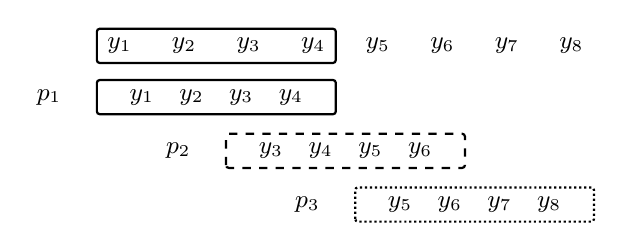
\begin{tikzpicture}[x=0.82cm,y=0.62cm,every node/.style={font=\small}]
  \foreach \i/\label in {0/{$y_1$},1/{$y_2$},2/{$y_3$},3/{$y_4$},4/{$y_5$},5/{$y_6$},6/{$y_7$},7/{$y_8$}} {
    \node[minimum width=0.7cm,minimum height=0.45cm] at (\i,0) {\label};
  }
  \draw[thick,rounded corners=1pt] (-0.35,-0.35) rectangle (3.35,0.35);
  \node[anchor=east] at (-0.75,-1.05) {$p_1$};
  \draw[thick,rounded corners=1pt] (-0.35,-1.4) rectangle (3.35,-0.7);
  \node at (1.5,-1.05) {$y_1\quad y_2\quad y_3\quad y_4$};
  \node[anchor=east] at (1.25,-2.15) {$p_2$};
  \draw[thick,dashed,rounded corners=1pt] (1.65,-2.5) rectangle (5.35,-1.8);
  \node at (3.5,-2.15) {$y_3\quad y_4\quad y_5\quad y_6$};
  \node[anchor=east] at (3.25,-3.25) {$p_3$};
  \draw[thick,densely dotted,rounded corners=1pt] (3.65,-3.6) rectangle (7.35,-2.9);
  \node at (5.5,-3.25) {$y_5\quad y_6\quad y_7\quad y_8$};
\end{tikzpicture}
\caption{Пример перекрывающихся patch при длине фрагмента $p=4$ и шаге $s=2$.}
\end{figure}
Каждый patch затем превращается в вектор фиксированной размерности $d$:
\begin{equation}
  e_j = W_p p_j + b_p,
  \qquad
  W_p \in \mathbb{R}^{d \times p}.
\end{equation}
После этого к $e_j$ обычно добавляют positional embedding, потому что Transformer должен понимать порядок фрагментов внутри контекста.
В итоге входное контекстное окно из $k$ точек превращается в последовательность из $m$ patch-токенов:
\begin{equation}
  (y_{T-k+1}, \ldots, y_T)
  \longmapsto
  (e_1, \ldots, e_m).
\end{equation}
Если, например, $k=96$, $p=16$ и $s=8$, то вместо $96$ точек входного окна модель получает $11$ токенов.
Это сильно уменьшает стоимость self-attention, потому что она квадратично зависит от числа токенов.
При этом один token уже содержит локальную форму ряда: короткий рост, падение, фрагмент сезонной волны или скачок уровня.
Важно различать две нарезки.
Сначала весь ряд длины $T$ превращают в набор обучающих примеров: для разных моментов времени берут окно прошлого длины $k$ и соответствующий будущий горизонт.
Например, один пример может иметь вход $(y_{t-k+1}, \ldots, y_t)$ и target $(y_{t+1}, \ldots, y_{t+h})$.
Затем уже внутри каждого такого входного окна выполняют patching и получают последовательность длины $m$.
Именно с этой последовательностью длины $m$ работает Transformer-блок.
Поэтому архитектура модели задаётся для числа patch-токенов $m$, а не для длины всей исторической записи $T$.
При inference обычно берут последние $k$ наблюдений, превращают их в $m$ patch-токенов и по ним строят прогноз на горизонт $h$.
PatchTST показал, что для Transformer-моделей такой ход особенно полезен: patch сохраняет локальный паттерн, уменьшает число токенов и позволяет attention смотреть на более длинную историю при той же вычислительной цене \cite{nie2023patchtst}.
Похожие patch-based идеи используются и в современных forecasting foundation models, например TimesFM \cite{das2024timesfm}.
Параметры $p$ и $s$ являются частью inductive bias.
Маленький patch ближе к поточечной модели и лучше сохраняет мелкие изменения.
Большой patch агрессивнее сжимает историю и удобен для длинного контекста, но может сгладить быстрые локальные события.

\subsubsection{Квантованные токены}

Другой путь -- дискретизировать значения ряда и получить настоящие token embeddings.
Сначала значение обычно приводят к сопоставимому масштабу, потому что один и тот же словарь должен работать для рядов с разными уровнями:
\begin{equation}
  z_t = \frac{y_t}{a},
\end{equation}
где $a$ -- масштаб ряда или входного окна.
Например, $a$ можно взять как средний абсолютный уровень в контексте.
После этого числовую ось разбивают на $V$ интервалов:
\begin{equation}
  -\infty = b_0 < b_1 < \ldots < b_V = +\infty.
\end{equation}
Каждое нормированное значение $z_t$ заменяют индексом интервала:
\begin{equation}
  q_t = Q(z_t) = r
  \quad \text{если} \quad
  z_t \in [b_{r-1}, b_r).
\end{equation}
Теперь $q_t$ -- это уже дискретный токен из словаря размера $V$.
Дальше работает та же идея, что и в NLP:
\begin{equation}
  e_t = E[q_t].
\end{equation}
Матрица $E \in \mathbb{R}^{V \times d}$ хранит обучаемый embedding для каждого бина.
Тогда ряд становится похож на текстовую последовательность из дискретных токенов, и к нему можно применять language-model-like обучение.
Например, модель может по токенам прошлого оценивать распределение следующего токена:
\begin{equation}
  \mathbb{P}_\theta(q_{t+1} \mid q_1, \ldots, q_t).
\end{equation}
Loss в такой постановке становится обычной cross-entropy по словарю бинов:
\begin{equation}
  \mathcal{L}(\theta)
  =
  -\sum_t \log \mathbb{P}_\theta(q_{t+1} \mid q_1, \ldots, q_t).
\end{equation}
Для multi-step forecasting модель может порождать будущие токены autoregressive: сначала $\hat q_{T+1}$, затем $\hat q_{T+2}$ и так далее.
Чтобы вернуться к числовому прогнозу, токен переводят в representative value соответствующего интервала, например в середину бина:
\begin{equation}
  \hat z_t = c_{\hat q_t},
  \qquad
  \hat y_t = a \hat z_t.
\end{equation}
Если нужен probabilistic forecast, можно не брать один token, а сэмплировать несколько будущих token paths и затем деквантизовать их в числовые траектории.
Именно эта идея лежит в Chronos: значения ряда масштабируются, квантуются в фиксированный словарь, а затем модель обучается предсказывать токены будущих значений \cite{ansari2024chronos}.
Плюс такого подхода -- совместимость с мощными языковыми objective.
Минус -- потеря части точной числовой информации из-за квантования.
Грубые бины дают маленький словарь и более простую задачу классификации, но сильнее округляют значения.
Слишком мелкие бины лучше сохраняют числовую точность, зато увеличивают словарь и делают распределение по токенам более разреженным.

\subsubsection{Позиционные и временные embeddings}

Отдельный класс -- positional и temporal embeddings.
Поточечная проекция говорит, какое значение пришло на вход, но не говорит, где оно находится внутри окна.
Для RNN порядок частично задан самой рекуррентной обработкой.
Для Transformer это нужно добавлять явно, потому что self-attention без дополнительных признаков видит набор токенов, а не упорядоченную последовательность.
Если два значения одинаковы, то их value embedding тоже одинаков.
Но значение в начале окна и значение в конце окна должны восприниматься по-разному, потому что одно относится к более далёкому прошлому, а другое находится ближе к forecast origin.

Для этого к embedding токена добавляют позиционный вектор:
\begin{equation}
  \widetilde{e}_j = e_j + r_j,
\end{equation}
где $j$ -- номер токена внутри входного окна, а $r_j$ -- positional embedding этой позиции.
Если модель работает с patch-токенами, то $j$ нумерует patches, а не отдельные наблюдения.
Вектор $r_j$ может быть обучаемым параметром или фиксированной sinusoidal encoding, как в Transformer \cite{vaswani2017}.
В обоих случаях задача одна: дать модели информацию о порядке токенов.

\begin{figure}[!ht]
\centering
\begin{tikzpicture}[x=1.55cm,y=0.74cm,every node/.style={font=\small}]
  \foreach \i/\val/\pos/\tok in {0/{$y_{t-3}$}/{$r_1$}/{$\widetilde e_1$},1/{$y_{t-2}$}/{$r_2$}/{$\widetilde e_2$},2/{$y_{t-1}$}/{$r_3$}/{$\widetilde e_3$},3/{$y_t$}/{$r_4$}/{$\widetilde e_4$}} {
    \node[draw,rounded corners=1pt,minimum width=1.15cm,minimum height=0.48cm] at (\i,0) {\val};
    \node at (\i,-0.65) {$+$};
    \node[draw,dashed,rounded corners=1pt,minimum width=1.15cm,minimum height=0.48cm] at (\i,-1.3) {\pos};
    \node at (\i,-1.95) {$=$};
    \node[draw,rounded corners=1pt,minimum width=1.15cm,minimum height=0.48cm] at (\i,-2.6) {\tok};
  }
  \node[anchor=east] at (-0.7,0) {значение};
  \node[anchor=east] at (-0.7,-1.3) {позиция};
  \node[anchor=east] at (-0.7,-2.6) {токен};
\end{tikzpicture}
\caption{Позиционный embedding различает места токенов внутри входного окна.}
\end{figure}

У временных рядов есть ещё одна особенность: позиция в окне и календарное время -- разные вещи.
Позиция $j=4$ означает «четвёртый токен в текущем контексте».
Но календарный признак может означать «понедельник», «полночь», «декабрь» или «праздничный день».
Эти признаки помогают модели учить сезонность, которую трудно восстановить только из локальной формы ряда.
Например, одинаковое значение спроса утром и вечером может иметь разный смысл для прогноза.

Календарные признаки обычно кодируют отдельными embedding-таблицами:
\begin{equation}
  c_t =
  E_{\mathrm{hour}}[\mathrm{hour}(t)]
  +
  E_{\mathrm{dow}}[\mathrm{dow}(t)]
  +
  E_{\mathrm{month}}[\mathrm{month}(t)].
\end{equation}
После этого value embedding, positional embedding и temporal embedding объединяют сложением или конкатенацией:
\begin{equation}
  \widetilde{e}_t = e_t + r_t + c_t.
\end{equation}
Если используется конкатенация, то получившийся вектор обычно дополнительно пропускают через линейный слой, чтобы получить нужную размерность.

\begin{figure}[!ht]
\centering
\begin{tikzpicture}[x=1.8cm,y=0.68cm,every node/.style={font=\small}]
  \foreach \i/\val/\hour/\dow in {0/{$y_1$}/{09}/{Пн},1/{$y_2$}/{10}/{Пн},2/{$y_3$}/{11}/{Пн},3/{$y_4$}/{12}/{Пн}} {
    \node[draw,rounded corners=1pt,minimum width=1.18cm,minimum height=0.45cm] at (\i,0) {\val};
    \node[draw,dashed,rounded corners=1pt,minimum width=1.18cm,minimum height=0.45cm] at (\i,-0.85) {час \hour};
    \node[draw,dotted,rounded corners=1pt,minimum width=1.18cm,minimum height=0.45cm] at (\i,-1.7) {день \dow};
    \node at (\i,-2.35) {$\downarrow$};
    \node[draw,rounded corners=1pt,minimum width=1.18cm,minimum height=0.45cm] at (\i,-3.0) {$e_t+c_t$};
  }
  \node[anchor=east] at (-0.65,0) {ряд};
  \node[anchor=east] at (-0.65,-0.85) {время};
  \node[anchor=east] at (-0.65,-1.7) {календарь};
  \node[anchor=east] at (-0.65,-3.0) {embedding};
\end{tikzpicture}
\caption{Temporal embeddings добавляют к значениям ряда известную календарную семантику.}
\end{figure}

Time2Vec формализует похожую идею как модельно-независимое векторное представление времени, где часть координат линейна, а часть периодична \cite{kazemi2019time2vec}.
В простом виде это можно записать как
\begin{equation}
  \mathrm{Time2Vec}(\tau)
  =
  \left(
    \omega_0 \tau + \varphi_0,
    \sin(\omega_1 \tau + \varphi_1),
    \ldots,
    \sin(\omega_d \tau + \varphi_d)
  \right).
\end{equation}
Линейная координата помогает кодировать тренд времени, а периодические координаты помогают кодировать циклы.
Для временных рядов это естественно: час дня, день недели и годовая сезонность имеют периодическую структуру.

Важно только не допускать leakage.
В embedding можно включать лишь ту информацию о времени, которая известна в момент построения прогноза.
Например, час дня, день недели и номер месяца для будущих точек обычно известны заранее.
Но признак «будет ли аномальный всплеск спроса завтра» использовать нельзя, если в реальной задаче он неизвестен в forecast origin.

\subsubsection{Static и categorical embeddings}

В панельных задачах полезны static и categorical embeddings.
Если у нас есть много рядов одного типа, идентификатор товара, магазина, региона или датчика можно подать в обучаемую таблицу:
\begin{equation}
  a_i = E_{\mathrm{id}}[i].
\end{equation}
Такой вектор не заменяет историю ряда, но помогает глобальной модели различать объекты и переносить статистическую силу между похожими рядами.
Здесь $i$ -- индекс конкретного ряда в панели.
Например, в retail forecasting ряд может соответствовать паре «товар--магазин».
Тогда можно завести отдельные таблицы embeddings для товара и магазина:
\begin{equation}
  a_i =
  E_{\mathrm{item}}[\mathrm{item}(i)]
  +
  E_{\mathrm{store}}[\mathrm{store}(i)].
\end{equation}
Если есть регион, категория товара или тип датчика, их embeddings добавляют тем же способом или конкатенируют и затем проецируют линейным слоем.

Один из самых простых вариантов прокинуть такой static embedding -- повторить его для каждого временного токена.
Для поточечной токенизации это выглядит так:
\begin{equation}
  e_{i,t}^{\mathrm{value}} = W_y y_{i,t} + b_y,
\end{equation}
\begin{equation}
  \widetilde{e}_{i,t}
  =
  W_{\mathrm{in}}
  \left[
    e_{i,t}^{\mathrm{value}};
    r_t;
    c_t;
    a_i
  \right]
  +
  b_{\mathrm{in}}.
\end{equation}
Здесь $r_t$ отвечает за позицию внутри окна, $c_t$ -- за календарные признаки, а $a_i$ -- за свойства всего ряда.
Квадратные скобки означают конкатенацию признаков.
После такой проекции RNN, TCN или Transformer получает обычную последовательность токенов, но каждый токен уже «знает», к какому товару, магазину или датчику он относится.

В patch embeddings идея такая же.
Для ряда $i$ сначала строятся patch-токены:
\begin{equation}
  e_{i,j}^{\mathrm{patch}} = W_p p_{i,j} + b_p.
\end{equation}
Затем один и тот же static embedding $a_i$ добавляется ко всем patch-токенам этого ряда:
\begin{equation}
  \widetilde{e}_{i,j}
  =
  W_{\mathrm{in}}
  \left[
    e_{i,j}^{\mathrm{patch}};
    r_j;
    a_i
  \right]
  +
  b_{\mathrm{in}},
  \qquad
  j = 1, \ldots, m.
\end{equation}
То есть static embedding не создаёт отдельную временную динамику.
Он работает как условие, на фоне которого модель интерпретирует все patches данного ряда.

\begin{figure}[!ht]
\centering
\begin{tikzpicture}[x=1.85cm,y=0.72cm,every node/.style={font=\small}]
  \foreach \i/\patch in {0/{$p_1$},1/{$p_2$},2/{$p_3$}} {
    \node[draw,rounded corners=1pt,minimum width=1.25cm,minimum height=0.48cm] at (\i,0) {\patch};
    \node at (\i,-0.6) {$\downarrow$};
    \node[draw,dashed,rounded corners=1pt,minimum width=1.25cm,minimum height=0.48cm] at (\i,-1.2) {$e_j^{\mathrm{patch}}$};
    \node at (\i,-1.8) {$+$};
    \node[draw,dotted,rounded corners=1pt,minimum width=1.25cm,minimum height=0.48cm] at (\i,-2.4) {$a_i$};
    \node at (\i,-3.0) {$\downarrow$};
    \node[draw,rounded corners=1pt,minimum width=1.25cm,minimum height=0.48cm] at (\i,-3.6) {$\widetilde e_{i,j}$};
  }
  \node[anchor=west] at (3.0,-2.4) {$a_i$: товар, магазин, регион};
  \draw[->,thick] (2.8,-3.6) -- (3.55,-3.6);
  \node[anchor=west] at (3.65,-3.6) {Transformer / RNN};
\end{tikzpicture}
\caption{Static embedding одного ряда повторяется для всех patch-токенов этого ряда.}
\end{figure}

Есть и второй распространённый вариант: не добавлять $a_i$ к каждому входному токену, а использовать его в прогнозной голове.
Пусть encoder уже построил скрытое представление окна $h_i$.
Тогда прогноз можно строить по объединению динамического состояния и статического описания ряда:
\begin{equation}
  \widehat{y}_{i,t+1:t+h}
  =
  g_\theta([h_i; a_i]).
\end{equation}
Первый способ влияет на обработку всей последовательности с самого начала.
Второй способ оставляет encoder более универсальным, но даёт forecast head информацию о том, для какого объекта строится прогноз.
DeepAR использует static categorical features в глобальной autoregressive RNN, а Temporal Fusion Transformer строит отдельные компоненты для static inputs и temporal inputs \cite{salinas2017,lim2021tft}.
Ограничение очевидное: такие embeddings легко начинают запоминать конкретные объекты, поэтому validation должен проверять не только знакомые ряды, но и устойчивость к новым или редким объектам.

\subsubsection{Variate tokens}

Для multivariate series появляется ещё один выбор: токеном может быть не момент времени, а отдельная переменная.
В обычной токенизации модель видит последовательность моментов времени.
Если в каждый момент времени наблюдается $d$ переменных, то входное окно можно записать как матрицу
\begin{equation}
  Y_{t-k+1:t}
  =
  \begin{pmatrix}
    y_{t-k+1}^{(1)} & y_{t-k+1}^{(2)} & \cdots & y_{t-k+1}^{(d)} \\
    y_{t-k+2}^{(1)} & y_{t-k+2}^{(2)} & \cdots & y_{t-k+2}^{(d)} \\
    \vdots & \vdots & \ddots & \vdots \\
    y_t^{(1)} & y_t^{(2)} & \cdots & y_t^{(d)}
  \end{pmatrix}.
\end{equation}
Обычная time-token логика берёт строку этой матрицы и делает токеном момент времени:
\begin{equation}
  u_\tau =
  (y_\tau^{(1)}, \ldots, y_\tau^{(d)}).
\end{equation}
Тогда Transformer сравнивает между собой разные моменты времени.
Variate-token логика делает наоборот: берёт столбец матрицы и делает токеном всю историю одной переменной:
\begin{equation}
  v_\ell =
  (y_{t-k+1}^{(\ell)}, \ldots, y_t^{(\ell)}),
  \qquad
  \ell = 1, \ldots, d.
\end{equation}
После этого каждый столбец проектируется в embedding space:
\begin{equation}
  e_\ell = W_v v_\ell + b_v,
  \qquad
  W_v \in \mathbb{R}^{r \times k}.
\end{equation}
В результате входом Transformer становится не последовательность длины $k$, а последовательность длины $d$:
\begin{equation}
  (e_1, \ldots, e_d).
\end{equation}
То есть attention сравнивает не временные позиции, а переменные ряда.
iTransformer предлагает именно такую инверсию: рассматривать variates как токены, а историю каждой переменной -- как её embedding \cite{liu2024itransformer}.

\begin{figure}[!ht]
\centering
\begin{tikzpicture}[x=1cm,y=0.68cm,every node/.style={font=\small}]
  \foreach \row/\time in {0/{$t-3$},1/{$t-2$},2/{$t-1$},3/{$t$}} {
    \node[anchor=east] at (-1.0,-\row) {\time};
  }
  \foreach \x/\name in {0/{$y^{(1)}$},1.7/{$y^{(2)}$},3.4/{$y^{(3)}$}} {
    \node at (\x,0.82) {\name};
  }
  \foreach \row in {0,1,2,3} {
    \foreach \x in {0,1.7,3.4} {
      \node[draw,minimum width=0.78cm,minimum height=0.42cm] at (\x,-\row) {$y$};
    }
  }
  \draw[thick,rounded corners=1pt] (-0.52,0.35) rectangle (0.52,-3.35);
  \draw[thick,dashed,rounded corners=1pt] (1.18,0.35) rectangle (2.22,-3.35);
  \draw[thick,densely dotted,rounded corners=1pt] (2.88,0.35) rectangle (3.92,-3.35);
  \node at (0,-4.05) {$v_1$};
  \node at (1.7,-4.05) {$v_2$};
  \node at (3.4,-4.05) {$v_3$};
  \draw[->,thick] (4.45,-1.5) -- (5.25,-1.5);
  \node[anchor=west] at (5.4,-0.8) {токены};
  \node[anchor=west] at (5.4,-1.5) {переменных};
  \node[anchor=west] at (5.4,-2.2) {$(e_1,e_2,e_3)$};
\end{tikzpicture}
\caption{Variate tokens: каждый токен кодирует историю одной переменной внутри окна.}
\end{figure}

Например, в задаче энергопотребления переменными могут быть нагрузка, температура и влажность.
Time-token Transformer будет сравнивать час с часом, где каждый час содержит все переменные.
Variate-token Transformer будет сравнивать переменную «нагрузка» с переменной «температура» и переменной «влажность», причём каждая переменная представлена своим недавним профилем.
Такой подход полезен, когда главная структура задачи находится не только во времени, но и в зависимостях между переменными.
Например, модель может выучить, что одна переменная систематически опережает другую или что несколько датчиков движутся согласованно.

Прогнозная голова после Transformer обычно возвращает будущие значения для одной или нескольких переменных:
\begin{equation}
  \widehat{y}_{t+1:t+h}^{(1:d)}
  =
  g_\theta(H_1, \ldots, H_d),
\end{equation}
где $H_\ell$ -- выход encoder-а для variate token $\ell$.
Если нужно прогнозировать только целевой ряд, то head может брать только его представление $H_{\mathrm{target}}$ или агрегировать все $H_1,\ldots,H_d$.
Для одномерных рядов такой приём не нужен, потому что при $d=1$ attention между переменными исчезает.
Для сенсорных панелей, энергии или трафика он меняет сам вопрос о том, что именно модель должна сравнивать через attention.

\subsubsection{Latent representations}

Наконец, embedding можно не задавать вручную, а предварительно обучать как latent representation.
В masked-modeling подходах часть точек или patch-токенов скрывают, а encoder учится восстанавливать их по контексту.
Так устроены time-series representation модели на базе Transformer, например TST у Zerveas et al. \cite{zerveas2021}.
В contrastive learning строят два связанных вида одного фрагмента ряда и учат модель сближать их представления, отличая от других фрагментов.
Так работают TNC и TS2Vec, где representation можно получать для timestamp, окна или всей последовательности \cite{tonekaboni2021,yue2022ts2vec}.
Эти методы особенно полезны, когда размеченных forecasting-задач мало, но есть много неразмеченных исторических рядов.
Однако такой embedding не всегда оптимален именно для causal forecasting: pretext task может учить хорошее общее представление, но downstream head всё равно нужно проверять на честном прогнозном split.

\subsubsection{Практический выбор}

\begin{table}[!ht]
\centering
\begin{tabular}{p{0.24\linewidth}p{0.28\linewidth}p{0.34\linewidth}}
\hline
Подход & Что становится токеном & Когда полезен \\
\hline
Поточечная проекция & Одно значение $y_t$ & RNN/GRU/LSTM и простые Transformer-бейзлайны \\
Окно лагов & Последние $k$ значений & Короткая локальная динамика и autoregressive-интуиция \\
Patch embedding & Фрагмент из $p$ соседних значений & Длинный контекст и Transformer-модели \\
Квантованные токены & Бин значения ряда & Language-model-like обучение и foundation models \\
Temporal embedding & Позиция и календарное время & Сезонность и порядок внутри окна \\
Static embedding & Идентификатор ряда или объекта & Глобальные модели на множестве связанных рядов \\
Variate token & Отдельная переменная ряда & Multivariate зависимости между переменными \\
Latent representation & Вектор encoder-а для точки, окна или ряда & Self-supervised pretraining и transfer \\
\hline
\end{tabular}
\caption{Основные способы построить embeddings для временных рядов.}
\end{table}

Практически это означает, что перед выбором архитектуры нужно сначала решить, что модель будет считать элементом последовательности.
Для короткого горизонта и небольших данных часто достаточно поточечной проекции или окна лагов.
Для длинного контекста обычно сильнее patch embeddings.
Для множества связанных рядов важны static embeddings.
Для foundation-model-подходов всё чаще используют либо patches, либо дискретные tokens, либо предварительно обученные latent representations.

\subsection{Нормировка временных рядов}

Нормировка в deep forecasting -- это не косметический preprocessing, а часть постановки задачи.
Нейросеть обычно легче обучается, если входы имеют сопоставимый масштаб.
Но для временных рядов нормировка легко создаёт leakage: статистики преобразования могут нечаянно использовать будущее.
Общее правило такое: любые параметры preprocessing должны оцениваться только по той информации, которая была бы доступна в момент построения прогноза \cite{sklearnCommonPitfalls}.

\subsubsection{Где возникает leakage}

Пусть один ряд разбит на train и test:
\begin{equation}
  (y_1,\ldots,y_{T_{\mathrm{train}}})
  \quad\text{и}\quad
  (y_{T_{\mathrm{train}}+1},\ldots,y_T).
\end{equation}
Нечестный вариант -- сначала посчитать среднее и стандартное отклонение по всему ряду, а потом сделать split:
\begin{equation}
  \mu_{\mathrm{all}} = \frac{1}{T}\sum_{t=1}^{T} y_t,
  \qquad
  \sigma_{\mathrm{all}}^2 = \frac{1}{T}\sum_{t=1}^{T}(y_t-\mu_{\mathrm{all}})^2.
\end{equation}
После этого нормированный ряд
\begin{equation}
  \widetilde{y}_t =
  \frac{y_t-\mu_{\mathrm{all}}}{\sigma_{\mathrm{all}}+\varepsilon}
\end{equation}
уже содержит информацию из test-отрезка через $\mu_{\mathrm{all}}$ и $\sigma_{\mathrm{all}}$.
Проблема остаётся даже тогда, когда модель видит только train-окна.
Если прогноз в нормированном масштабе затем переводится обратно как
\begin{equation}
  \widehat{y}_{t+1:t+h}
  =
  (\sigma_{\mathrm{all}}+\varepsilon)\widehat{\widetilde{y}}_{t+1:t+h}
  +
  \mu_{\mathrm{all}},
\end{equation}
то обратная нормировка тоже использует будущий test-отрезок.
Поэтому честный pipeline сначала фиксирует временной split, потом оценивает scaler на train-части, а затем применяет его к train, validation и test:
\begin{equation}
  \mu_{\mathrm{train}} = \frac{1}{T_{\mathrm{train}}}\sum_{t=1}^{T_{\mathrm{train}}} y_t,
  \qquad
  \sigma_{\mathrm{train}}^2 =
  \frac{1}{T_{\mathrm{train}}}\sum_{t=1}^{T_{\mathrm{train}}}(y_t-\mu_{\mathrm{train}})^2.
\end{equation}
Тогда
\begin{equation}
  \widetilde{y}_t =
  \frac{y_t-\mu_{\mathrm{train}}}{\sigma_{\mathrm{train}}+\varepsilon},
  \qquad
  \widehat{y}_{t+1:t+h}
  =
  (\sigma_{\mathrm{train}}+\varepsilon)\widehat{\widetilde{y}}_{t+1:t+h}
  +
  \mu_{\mathrm{train}}.
\end{equation}
В rolling-origin evaluation это правило применяется к каждому origin отдельно.
Если прогноз строится из точки $\tau$, то допустимы только статистики, вычисленные по наблюдениям не позже $\tau$.
Использовать $y_{\tau+1},\ldots,y_{\tau+h}$ нельзя, потому что это уже target прогноза.

\subsubsection{Локальные модели}

Локальная модель обучается для одного ряда или для небольшой группы рядов независимо от остальных.
В этом случае нормировку обычно считают отдельно для каждого ряда по его обучающей истории:
\begin{equation}
  \widetilde{y}_{i,t}
  =
  \frac{y_{i,t}-\mu_{i,\mathrm{train}}}{\sigma_{i,\mathrm{train}}+\varepsilon}.
\end{equation}
Здесь $i$ -- индекс ряда, а $\mu_{i,\mathrm{train}}$ и $\sigma_{i,\mathrm{train}}$ считаются только по train-части этого ряда.
Такой подход сохраняет честность evaluation и делает оптимизацию стабильнее.
Если ряд нестационарен, scaler можно обновлять во времени, но только причинно: на origin $\tau$ он должен зависеть от $y_{i,1:\tau}$, а не от будущего.
Например, можно использовать среднее и стандартное отклонение по последнему известному окну:
\begin{equation}
  \mu_{i,\tau}^{(k)} =
  \frac{1}{k}\sum_{j=0}^{k-1} y_{i,\tau-j},
  \qquad
  \sigma_{i,\tau}^{(k)}
  =
  \sqrt{
    \frac{1}{k}\sum_{j=0}^{k-1}
    (y_{i,\tau-j}-\mu_{i,\tau}^{(k)})^2
  }.
\end{equation}
Тогда модель прогнозирует нормированные будущие значения, а обратное преобразование использует те же статистики последнего известного окна.
Это похоже на идею reversible instance normalization: нормировать каждый входной instance по его контексту, а выход модели возвращать в исходный масштаб теми же статистиками \cite{kim2022revin}.

\subsubsection{Глобальные модели}

Глобальная модель обучается сразу на коллекции рядов.
Здесь нормировка становится особенно важной: если ряды имеют разный масштаб, то крупные ряды могут доминировать в loss, а маленькие будут почти незаметны.
В DeepAR эта проблема явно выделена как одна из трудностей обучения на больших панелях, и используется item-dependent scaling: для каждого ряда вводится собственный масштаб, а модель обучается на приведённых значениях \cite{salinas2017}.
В простом варианте можно взять
\begin{equation}
  a_i =
  \frac{1}{T_{i,\mathrm{train}}}
  \sum_{t \in \mathcal{T}_{i,\mathrm{train}}}
  |y_{i,t}|
  +
  \varepsilon,
  \qquad
  \widetilde{y}_{i,t} = \frac{y_{i,t}}{a_i}.
\end{equation}
После прогноза нормированного ряда обратное преобразование делается как
\begin{equation}
  \widehat{y}_{i,t+1:t+h}
  =
  a_i \widehat{\widetilde{y}}_{i,t+1:t+h}.
\end{equation}
Такой scaler считается по каждому ряду отдельно, но сама нейросеть имеет общие параметры для всей панели.
То есть масштабы $a_i$ разные для разных рядов, а веса модели $\theta$ одни и те же для всех обучающих окон.
Это хороший вариант для demand forecasting, трафика, метрик и сенсоров, где форма динамики похожа, а абсолютные уровни отличаются на порядки.
Например, пусть один ряд описывает продажи популярного товара с уровнем около $1000$ штук в день, а другой -- редкого товара с уровнем около $5$ штук в день.
Без нормировки ошибка в $100$ штук на первом товаре может оказаться для loss важнее, чем ошибка в $5$ штук на втором, хотя для редкого товара это уже огромная относительная ошибка.
Per-series scaling приводит оба ряда к сопоставимому масштабу, но не заставляет модель забыть, что товары разные.
Сам масштаб $a_i$ можно дополнительно подать в модель как static feature или использовать только на этапе обратного преобразования.

Второй вариант -- считать общие статистики по всей train-панели.
Здесь мы объединяем все наблюдения из всех рядов в один большой набор и считаем одно среднее и одно стандартное отклонение:
\begin{equation}
  \mu_{\mathrm{panel}}
  =
  \frac{1}{N_{\mathrm{train}}}
  \sum_i \sum_{t \in \mathcal{T}_{i,\mathrm{train}}} y_{i,t},
  \qquad
  \sigma_{\mathrm{panel}}^2
  =
  \frac{1}{N_{\mathrm{train}}}
  \sum_i \sum_{t \in \mathcal{T}_{i,\mathrm{train}}}
  (y_{i,t}-\mu_{\mathrm{panel}})^2.
\end{equation}
Здесь $N_{\mathrm{train}}$ -- общее число train-наблюдений во всей панели, то есть сумма длин train-частей всех рядов.
После этого каждое значение любого ряда нормируется одинаково:
\begin{equation}
  \widetilde{y}_{i,t}
  =
  \frac{y_{i,t}-\mu_{\mathrm{panel}}}{\sigma_{\mathrm{panel}}+\varepsilon}.
\end{equation}
Такой подход сохраняет информацию об относительных уровнях между рядами.
Если ряд $A$ в десять раз выше ряда $B$, то после общей нормировки это различие всё ещё видно модели.
Это может быть полезно, когда абсолютный уровень сам является содержательным сигналом.
Например, если несколько датчиков одного типа измеряют температуру в разных точках одной системы, то разница уровней между датчиками может говорить о реальном пространственном градиенте.
Но для неоднородной панели общий scaler часто хуже.
Если в одной панели лежат маленькие магазины и федеральные хиты продаж, то среднее и дисперсия панели будут в основном определяться крупными рядами.
Мелкие ряды после такой нормировки окажутся сжаты около нуля, и модель может начать хуже различать их локальную динамику.

Третий вариант -- считать статистики по группам.
Он находится между per-series scaling и одним общим scaler-ом.
Пусть каждый ряд относится к группе $g(i)$: категории товара, региону, типу датчика или частоте наблюдений.
Тогда для каждой группы считаются свои статистики только по train-наблюдениям рядов этой группы:
\begin{equation}
  \mu_{g,\mathrm{train}}
  =
  \frac{1}{N_{g,\mathrm{train}}}
  \sum_{i:g(i)=g}
  \sum_{t \in \mathcal{T}_{i,\mathrm{train}}}
  y_{i,t},
\end{equation}
\begin{equation}
  \sigma_{g,\mathrm{train}}^2
  =
  \frac{1}{N_{g,\mathrm{train}}}
  \sum_{i:g(i)=g}
  \sum_{t \in \mathcal{T}_{i,\mathrm{train}}}
  (y_{i,t}-\mu_{g,\mathrm{train}})^2.
\end{equation}
Затем ряд $i$ нормируется статистиками своей группы:
\begin{equation}
  \widetilde{y}_{i,t}
  =
  \frac{y_{i,t}-\mu_{g(i),\mathrm{train}}}{\sigma_{g(i),\mathrm{train}}+\varepsilon}.
\end{equation}
Например, товары внутри одной категории можно привести к общему масштабу категории, но не смешивать молоко, смартфоны и зимние куртки в один scaler.
Так модель сохраняет часть межсерийной информации внутри группы, но не страдает от слишком грубого общего масштаба.

Для multivariate forecasting похожая идея применяется по переменным.
Если в одном окне есть нагрузка, температура и влажность, то это не три ряда в одном масштабе, а три разные физические величины.
Поэтому часто считают отдельный scaler для каждой переменной $\ell$:
\begin{equation}
  \widetilde{y}_{i,t}^{(\ell)}
  =
  \frac{y_{i,t}^{(\ell)}-\mu_{\ell,\mathrm{train}}}{\sigma_{\ell,\mathrm{train}}+\varepsilon}.
\end{equation}
Здесь $\mu_{\ell,\mathrm{train}}$ и $\sigma_{\ell,\mathrm{train}}$ считаются по train-части переменной $\ell$.
Если данных много и переменная наблюдается для многих объектов, статистики можно считать по всем объектам, но только для этой переменной.
Например, отдельный scaler для температуры не должен использовать значения нагрузки, а scaler для нагрузки не должен использовать влажность.
Главное условие остаётся тем же: все $\mu$ и $\sigma$ оцениваются только по train-части соответствующей группы.

\subsubsection{Что выбрать на практике}

\begin{table}[!ht]
\centering
\begin{tabular}{p{0.24\linewidth}p{0.34\linewidth}p{0.28\linewidth}}
\hline
Сценарий & Нормировка & На что смотреть \\
\hline
Один ряд & Scaler по train-части ряда & Не использовать будущий test при обратном преобразовании \\
Много рядов разного масштаба & Per-series scale $a_i$ & Масштаб можно подать как static feature \\
Однородная панель & Общий train-scaler & Проверить, не доминируют ли крупные ряды в loss \\
Multivariate ряд & Scaler по каждой переменной & Не смешивать переменные с разными единицами \\
Сильный drift & Window/instance normalization & Считать статистики только по известному контексту \\
\hline
\end{tabular}
\caption{Типовые варианты нормировки временных рядов без leakage.}
\end{table}

Практическое правило можно сформулировать так.
Если модель локальная, начинаем со scaler-а по train-части данного ряда.
Если модель глобальная и ряды отличаются масштабом, начинаем с per-series scaling.
Если ряды однородны и абсолютные уровни между ними сопоставимы, можно проверить общий scaler по панели.
Если распределение заметно меняется во времени, полезно добавить causal window normalization или RevIN-подобный слой.
Во всех случаях scaler, обратное преобразование и validation protocol должны быть частью одного воспроизводимого pipeline, а не отдельной ручной операцией после обучения.

\subsection{TCN}


\subsection{Transformer}


\newpage
\begin{thebibliography}{99}
\bibitem{arora2024}
Arora T.
The Many Faces of RNNs: Understanding Different Architectures.
LinkedIn, 2024.
\url{https://www.linkedin.com/pulse/many-faces-rnns-understanding-different-architectures-tarun-arora-grxpf}.

\bibitem{bentaieb2012}
Ben Taieb S., Bontempi G., Atiya A. F., Sorjamaa A.
A review and comparison of strategies for multi-step ahead time series forecasting based on the NN5 forecasting competition.
Expert Systems with Applications, 2012.
\url{https://doi.org/10.1016/j.eswa.2012.01.039}.

\bibitem{wen2017}
Wen R., Torkkola K., Narayanaswamy B., Madeka D.
A Multi-Horizon Quantile Recurrent Forecaster.
NIPS Time Series Workshop, 2017.
\url{https://arxiv.org/abs/1711.11053}.

\bibitem{salinas2017}
Salinas D., Flunkert V., Gasthaus J.
DeepAR: Probabilistic Forecasting with Autoregressive Recurrent Networks.
arXiv, 2017.
\url{https://arxiv.org/abs/1704.04110}.

\bibitem{sklearnCommonPitfalls}
Scikit-learn developers.
Common pitfalls and recommended practices.
Scikit-learn documentation.
\url{https://scikit-learn.org/stable/common_pitfalls.html}.

\bibitem{wikimediaBPTTUnfold}
Headlessplatter.
Unfold through time.png.
Wikimedia Commons, public domain, 2010.
\url{https://commons.wikimedia.org/wiki/File:Unfold_through_time.png}.

\bibitem{hochreiter1997}
Hochreiter S., Schmidhuber J.
Long Short-Term Memory.
Neural Computation, 1997.
\url{https://www.bioinf.jku.at/publications/older/2604.pdf}.

\bibitem{gers2000}
Gers F. A., Schmidhuber J., Cummins F.
Learning to Forget: Continual Prediction with LSTM.
Neural Computation, 2000.
\url{https://pubmed.ncbi.nlm.nih.gov/11032042/}.

\bibitem{jozefowicz2015}
Jozefowicz R., Zaremba W., Sutskever I.
An Empirical Exploration of Recurrent Network Architectures.
ICML, 2015.
\url{https://proceedings.mlr.press/v37/jozefowicz15.html}.

\bibitem{tallec2018}
Tallec C., Ollivier Y.
Can Recurrent Neural Networks Warp Time?
ICLR, 2018.
\url{https://openreview.net/forum?id=SJcKhk-Ab}.

\bibitem{cho2014}
Cho K., van Merrienboer B., Gulcehre C., Bahdanau D., Bougares F., Schwenk H., Bengio Y.
Learning Phrase Representations using RNN Encoder-Decoder for Statistical Machine Translation.
EMNLP, 2014.
\url{https://aclanthology.org/D14-1179/}.

\bibitem{chung2014}
Chung J., Gulcehre C., Cho K., Bengio Y.
Empirical Evaluation of Gated Recurrent Neural Networks on Sequence Modeling.
arXiv, 2014.
\url{https://arxiv.org/abs/1412.3555}.

\bibitem{olah2017habr}
Olah C.
LSTM -- сети долгой краткосрочной памяти.
Перевод на Хабре, 2017.
\url{https://habr.com/ru/companies/wunderfund/articles/331310/}.

\bibitem{vaswani2017}
Vaswani A., Shazeer N., Parmar N., Uszkoreit J., Jones L., Gomez A. N., Kaiser L., Polosukhin I.
Attention Is All You Need.
NeurIPS, 2017.
\url{https://arxiv.org/abs/1706.03762}.

\bibitem{kazemi2019time2vec}
Kazemi S. M., Goel R., Eghbali S., Ramanan J., Sahota J., Thakur S., Wu S., Smyth C., Poupart P., Brubaker M.
Time2Vec: Learning a Vector Representation of Time.
arXiv, 2019.
\url{https://arxiv.org/abs/1907.05321}.

\bibitem{lim2021tft}
Lim B., Arik S. O., Loeff N., Pfister T.
Temporal Fusion Transformers for interpretable multi-horizon time series forecasting.
International Journal of Forecasting, 2021.
\url{https://doi.org/10.1016/j.ijforecast.2021.03.012}.

\bibitem{nie2023patchtst}
Nie Y., Nguyen N. H., Sinthong P., Kalagnanam J.
A Time Series is Worth 64 Words: Long-term Forecasting with Transformers.
ICLR, 2023.
\url{https://arxiv.org/abs/2211.14730}.

\bibitem{das2024timesfm}
Das A., Kong W., Sen R., Zhou Y.
A decoder-only foundation model for time-series forecasting.
ICML, 2024.
\url{https://arxiv.org/abs/2310.10688}.

\bibitem{ansari2024chronos}
Ansari A. F., Stella L., Turkmen C., Zhang X., Mercado P., Shen H., Shchur O., Rangapuram S. S., Pineda Arango S., Kapoor S., Zschiegner J., Maddix D. C., Mahoney M. W., Torkkola K., Gordon Wilson A., Bohlke-Schneider M., Wang Y.
Chronos: Learning the Language of Time Series.
arXiv, 2024.
\url{https://arxiv.org/abs/2403.07815}.

\bibitem{liu2024itransformer}
Liu Y., Hu T., Zhang H., Wu H., Wang S., Ma L., Long M.
iTransformer: Inverted Transformers Are Effective for Time Series Forecasting.
ICLR, 2024.
\url{https://arxiv.org/abs/2310.06625}.

\bibitem{zerveas2021}
Zerveas G., Jayaraman S., Patel D., Bhamidipaty A., Eickhoff C.
A Transformer-based Framework for Multivariate Time Series Representation Learning.
KDD, 2021.
\url{https://arxiv.org/abs/2010.02803}.

\bibitem{tonekaboni2021}
Tonekaboni S., Eytan D., Goldenberg A.
Unsupervised Representation Learning for Time Series with Temporal Neighborhood Coding.
ICLR, 2021.
\url{https://arxiv.org/abs/2106.00750}.

\bibitem{yue2022ts2vec}
Yue Z., Wang Y., Duan J., Yang T., Huang C., Tong Y., Xu B.
TS2Vec: Towards Universal Representation of Time Series.
AAAI, 2022.
\url{https://arxiv.org/abs/2106.10466}.

\bibitem{kim2022revin}
Kim T., Kim J., Tae Y., Park C., Choi J.-H., Choo J.
Reversible Instance Normalization for Accurate Time-Series Forecasting against Distribution Shift.
ICLR, 2022.
\url{https://openreview.net/forum?id=cGDAkQo1C0p}.

\bibitem{lai2018}
Lai G., Chang W.-C., Yang Y., Liu H.
Modeling Long- and Short-Term Temporal Patterns with Deep Neural Networks.
SIGIR, 2018.
\url{https://arxiv.org/abs/1703.07015}.

\bibitem{pascanu2013}
Pascanu R., Mikolov T., Bengio Y.
On the difficulty of training recurrent neural networks.
ICML, 2013.
\url{https://proceedings.mlr.press/v28/pascanu13.html}.

\bibitem{smyl2020}
Smyl S.
A hybrid method of exponential smoothing and recurrent neural networks for time series forecasting.
International Journal of Forecasting, 2020.
\url{https://doi.org/10.1016/j.ijforecast.2019.03.017}.

\bibitem{hewamalage2021}
Hewamalage H., Bergmeir C., Bandara K.
Recurrent Neural Networks for Time Series Forecasting: Current status and future directions.
International Journal of Forecasting, 2021.
\url{https://doi.org/10.1016/j.ijforecast.2020.06.008}.

\end{thebibliography}

\end{document}
